\clearpage
\subsection{Blockchain}
\label{estatArt:blockchain}
%Blockchain és una estructura de dades ordenada, una llista de blocs de transaccions on cada bloc, es troba ellaçat amb el seu anterior.
%\newline Es pot enmagatzemar en un arxiu de text pla, així com en una base de dades simple. Els “Bitcoin core clients” enmagatzemen les metadades de la blockchain emprant els sistema de base de dades LavelDB de Google. Els blocs tenen un enllaç enrere, fent referència al seu bloc previ dins de la cadena.\\
%\newline Generalment, es visualitza el concepte de blockchain com una pila vertical; la visualització dels blocn empilats, un a sobre de l’altre, resulta en l’ús del terme “height” (alçada) per a referir-se a la distància entre el primer i l’últim bloc, i “top” o bé “tip” per afer referència a l’últim bloc que ha passat a formar part de la blockchain.\\
%\newline Cada bloc dins de la blockchain s’identifica amb un \textit{hash}; aquest es genera mitjançant mitjançant l’algorisme criptogràfic SHA256, a la capçalera. Cada bloc a més, fa referècia a l’anterior, conegut com a “parent block” mitjançant el camp “previous block \textit{hash}” de la capçalera del bloc. En altres paraules, cada bloc conté el \textit{hash} corresponent al seu pare dins de la seva capçalera. la seqüència de \textit{hash} que linquen cada block amb el seu pare, crea una cadena cap enradere fins a arribar al primer bloc creat, conegut com a “genesis block”.\\
%\newline Tot i que un block sols té un pare, temporalment pot tenir multiples fills; cadescún dels fills fa referència al mateix bloc com el seu pare i té el mateix \textit{hash} (el del pare) dins del camp “previous block \textit{hash}” de la seva capçalera. Aquest cas, es dona en el moment que es fa un fork a la blockchain, una situació de caire temporal que es produeix quan es descobreixen diversos blocs de forma simulània per diferents miners.\\
%Finalment, només un dels blocs passarà a formar part de la lockchain, i el “fork” quedarà resolt. Tot i que els blocs puguin tenir un o més fills, cada bloc disposa d’un únic pare. Això es deu a que un bloc té un únic camp “previous block \textit{hash}” referenciant al seu únic pare.\\
%\newline El camp “previous block \textit{hash}” es troba dins de la capcelera del bloc i, afectant directament al \textit{hash} dels blocs fills. La identitat d’un bloc fill canvia si la identitat del pare ho fa; és a dir, quan el pare és modificat, el seu \textit{hash} canvia i inevitablement l’apuntador (“previous block \textit{hash}”) del bloc fill s’ha de modificar amb el nou \textit{hash} del pare. Aquest canvi, alhora provoca que el \textit{hash} del bloc nét es veig també modificat i així succesivament. Aquest efecte cascada asseura que un cop un bloc té diverses generacions que el segueixen, no pot ser canviat sense haver de forçar el recalculat de cadescún dels \textit{hash} dels blocs sunsegüents. Aquest tipus de re-calculat, requereix d’una capacitat de computació molt gran, la existència d’una llarga cadena de blocs fa que la història de la blockchain sigui in-mutable; la qual cosa es converteix en una de les seves principals característiques a nivell de seguretat.

%\subsubsection{Estructura del bloc}
%Un bloc és una estructura de dades que agrega transaccions per a incloure-les a una espècie de llibre de comptes de caràcter públic, la blockchain. El block està format per una capçalera, on es guarden metadades, seguit d’una llarga llista de transaccions (que formen el gruix principal del bloc). \\
%\newline La capçalera ocupa 80 bytes fixes, mentre que una transacció de mitjana pesa com a mínim uns 250 bytes i un bloc de promig conté més de 500 transaccions.\\
%\newline A la següent taula es pot veure més detalladament l'estructura general d'un bloc:
%\begin{table}[ht]
%    \centering
%    \begin{tabular}{|l|l|l|} 
%    \hline
%    \textbf{Mida} & \textbf{Camp} & \textbf{Descripció} \\ [0.2ex] 
%    4 bytes & Block size & La mida del bloc que segueix aquest camp, en bytes \\
%    80 bytes & Block header & Camps corresponents a la capçalera  \\
%    1-9 bytes & Transacion counter & Quantes transaccions segueixen \\
%    Variable & Transactions & Transaccions registrades en el bloc  \\[0.1ex] 
%    \hline
%    \end{tabular}
%    \caption{Estructura general d'un bloc}
%    \label{block_structure}
%\end{table}

%\subsubsection{Capçalera del bloc}
%La capçalera del bloc està formada per tres bloc de metadades: 
%\begin{itemize}
%    \item Un primer bloc amb una referència al \textit{hash} del bloc anterior, que conecta el bloc en qüestió amb el seu anterior dins de la cadena
%    \item  Un segon bloc de metadades que fa referència a temes de mineria de bitcoin
%    \item Un tercer bloc correponent a l’arrel del “merkle tree”, una estuctura de dades per agregar de formaeficient les transaccions del bloc.
%\end{itemize}

%\subsubsection{Identificadors de bloc: \textit{hash} de capçalera i altura del bloc}
%El primer identificador d’un bloc es el seu \textit{hash}, una emprempta digital, generada a partir de realitzar el \textit{hash} (SHA256) de la capçalera 2 vegades. El resultat és un \textit{hash} de 32 bytes anomenat \textit{block \textit{hash}}, tot i que seria més correcte anomenar-lo “block header \textit{hash}”, ja que per a calcular-lo es fa servir únicament la capçalera del bloc. Un \textit{block \textit{hash}} identifica de forma inequívoca i única cada bloc.\\
%\newline Cal notar que aquest \textit{hash} no s’inclou dins del que s’anomena “block’s data structure”, tampoc quan es transmet el block per la xarxa ni quan es persisteix el bloc i passa a formar part de la blockchain. Per contra, cada node calcula aquest \textit{hash} en el moment en el rep el bloc a través de la xarxa. El \textit{block \textit{hash}} es guarda en una base de dades separada com part de les metadades del bloc, per tal de facilitar-ne la indexació i l’accés als bloc del disc.\\
%\newline Una segona forma d’identificar els blocs és mitjançant la seva posició dins de la blockchain, aquesta posició rep el nom d’altura. El primer bloc creat té altura 0. 
%Així doncs, un bloc es pot identificar tant per el seu \textit{block \textit{hash}} o bé per l’altura dins de la blockchain. Cada block afegit sobre aquest primer bloc, afegeix 1 a l’altura de la blockchain. Segons blockchain.info, l’altura de la cadena a data de 21 de Desembre de 2016, és de 444495 blocs, des de gener de 2009.\\
%\newline Cal tenir en compte però, que així com el \textit{block \textit{hash}} és únic per a cada bloc, l’altura no ho és; es poden donar situacions en que més d’un bloc competeixi per la mateixa posició dins de la blockchain. \\
%De la mateixa manera que el \textit{block \textit{hash}}, l’altura és una dada que no forma part de l’estructura de dades del bloc ni s’enmagatzema dins del bloc, sino que cada node calcula de forma dinàmica l’altura del bloc en el moment en el que es rep a través de la xarxa. Igual que el \textit{block \textit{hash}}, l’altura es guarda en una base de dades de metadades.
Una forma de d’entendre la \textit{blockchain}\cite{blockchain} és pensar en un gran llibre de comptes de caràcter públic, on cada transacció que s’efectua queda registrada i on tots els usuaris en tenen accés.
En termes més tècnics, \textit{blockchain} és una llista ordenada, una llista de blocs de transaccions on cada bloc, es troba enllaçat amb el bloc anterior.\\
\newline Generalment, es representa com una pila vertical, per tal d’ajudar a l’hora de definir termes com \textbf{alçada} (\textit{height}), corresponent al total de blocs de la cadena, i al \textbf{\textit{top}}, fet servir per indicar quin es l'últim bloc que ha passat a formar part de la cadena, i que com a conseqüència es troba al cap de munt de la pila representada.\\
\newline Cada bloc dins de la cadena té un identificador, un \textit{hash} generat a partir del contingut de la seva capçalera. Aquest identificador, és el que trobarem dins del camp \textit{previous block hash} del bloc fill.
Seguint els diferents \textit{previous block hash}  de cada element de la cadena, podriem arribar fins al primer bloc, que rep el nom de \textit{genesis block}.\\
\begin{wrapfigure}{r}{0.25\textwidth}
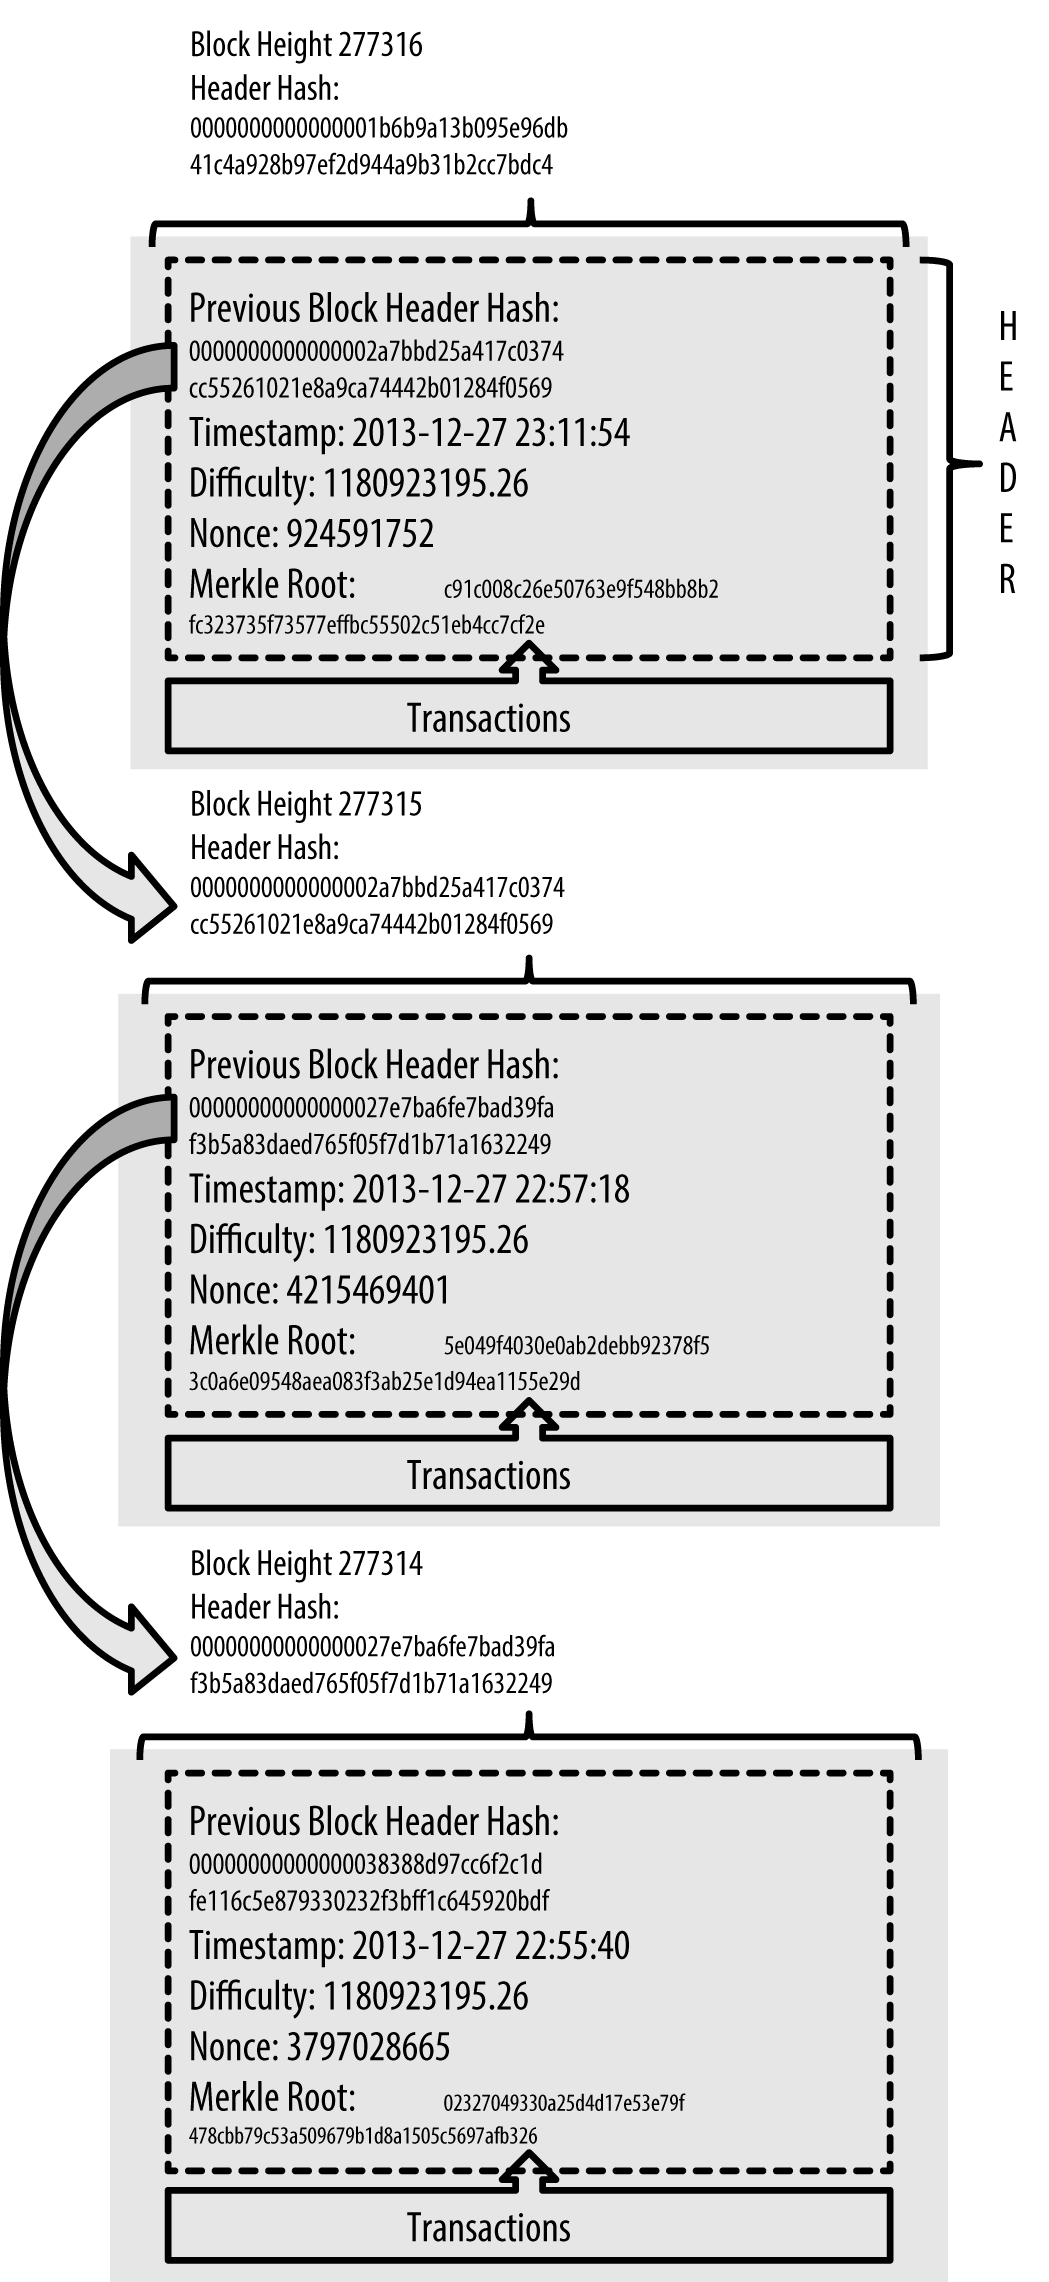
\includegraphics[scale=0.8]{sections/arquitectura/blockchain_diagram.png}
\caption{Blockchain}
\label{fig:blockchain}
\end{wrapfigure}
\newline Una de les característiques principals de \textit{blockchain}, i la que més rellevància té dins del projecte que ens ocupa, és la inmutabilitat de les dades, i en cas de trobar-se un canvi forçós, la facilitat a l’hora de trobar-ne l’origen.\\
\newline Aquesta característica deu el seu origen a la capçalera de cada un dels blocs que formen la cadena.
Dins d’aquesta capçalera, com s'ha dit anteriorment, es troba el camp \textit{previous block hash} que apunta al bloc  anterior, o el que és el mateix, el bloc pare.\\
\newline Fent un resum curt del contingut de la capçalera, trobem aquests tres elements:
\begin{itemize}
    \item Apuntador al bloc anterior (\textit{previous block hash})
    \item Metadades sobre mineria de blocs
    \item \textit{Hash} generat a partir de totes les transaccions registrades al bloc
\end{itemize}
Quan qualsevol dels tres camps que formen la capçalera d’un bloc es veu modificat, l’identificador d'aquest queda modificat, i com a conseqüència, el camp \textit{previous block hash} de la capçalera del fill, fent que l’identificador de bloc del fill es modifiqui, i així successivament fins a replicar-se a tots els nodes de la cadena.\\
\newline Aquesta petita modificació desencadena una successió de canvis a la \textit{blockchain} que requereix d’una capacitat de càlcul molt gran, i és fàcilment detectable.